% 03-data-exploration-and-pre-processing.tex

% Data Exploration and Pre-processing
% 3.1. Introduction: Introduces the data exploration and pre-processing tasks.
% 3.2. Dataset Preparation: Describes the process of loading the dataset and initial inspection.
% 3.3. Temporal Analysis: Analyzes when the attacks were performed.
% 3.4. Feature Extraction: Extracts features from the attack sessions.
% 3.5. Common Words Analysis: Identifies the most common words in the sessions.
% 3.6. Intent Distribution: Analyzes the distribution of intents over time.
% 3.7. Text Representation: Converts text into numerical representations (BoW, TF-IDF).

% Section Title
\section{DATA EXPLORATION AND PRE-PROCESSING}

    % Main Content

    \subsection{Introduction}
        
        This section outlines the steps taken to explore and preprocess the dataset used in this study. The primary objective is to understand the data characteristics, identify patterns, and prepare the data for further analysis. We focus on temporal trends, intent distributions, and textual features.
        
    \subsection{Dataset Overview}
    
        The dataset consists of logs from SSH attacks. Each entry includes the following features:

        \begin{itemize}
            \item \textbf{session\_id}: An integer representing the unique identifier for each session.
            \item \textbf{full\_session}: A string containing the full sequence of commands executed during the attack session.
            \item \textbf{first\_timestamp}: The timestamp indicating the start of the session.
            \item \textbf{Set\_Fingerprint}: A set of strings (labels) describing the nature of the attack.
        \end{itemize}

        Below is an example of the dataset structure:

        \begin{figure}[h!]
            \centering
            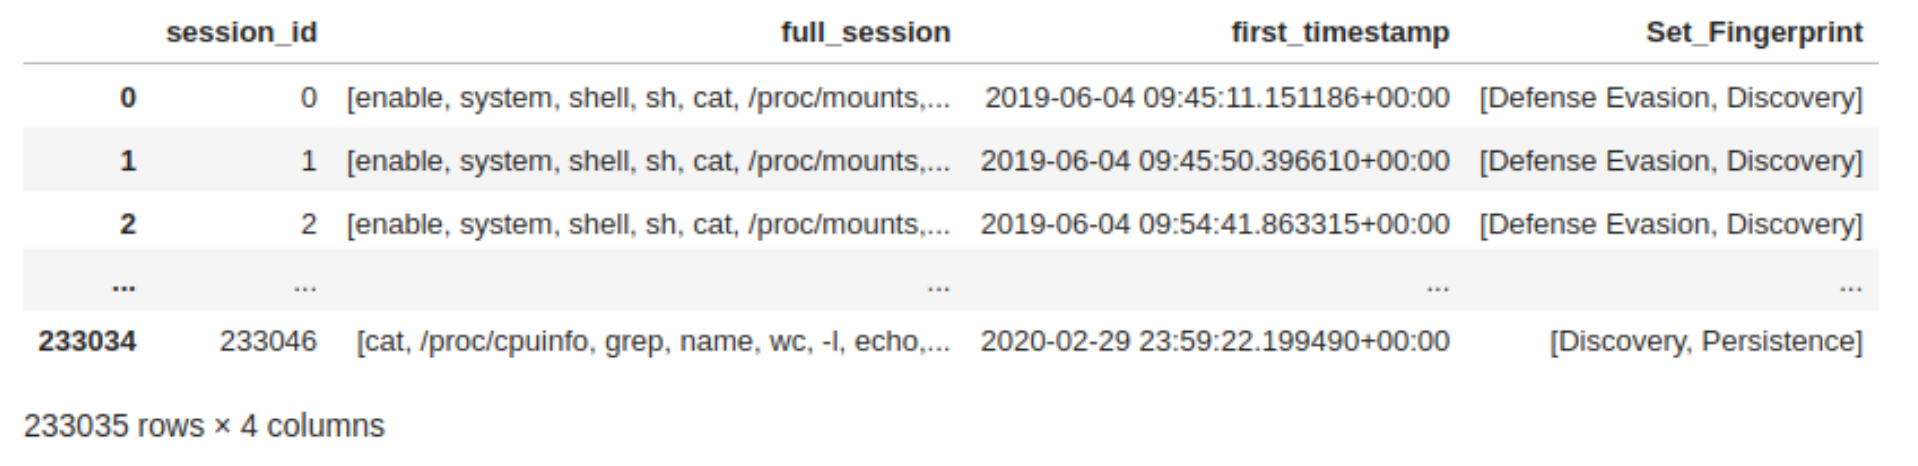
\includegraphics[width=0.9\textwidth]{figures/others/dataset_1.png}
            \vspace{-1em}
            \caption{Dataset}
            \label{fig:dataset_example}
        \end{figure}

    \vspace{-1em}

    \subsection{Dataset Preparation and Feature Extraction}

        The dataset used in this study was provided as a Parquet file.

        To prepare the dataset for analysis and ensure its quality, several preprocessing steps were undertaken, described in detail below:

        \begin{enumerate}
        
            \item \textbf{Decoding the \textbf{full\_session} column}: The \texttt{full\_session} column contained \texttt{90026} encoded shell scripts, making the raw data difficult to interpret. A decoding process was applied to these entries, converting them into a human-readable format.
            
            \vspace{0.2em}
            
            \item \textbf{Formatting the \textbf{first\_timestamp} column}: The \texttt{first\_timestamp} column was checked for consistency and converted into a standard datetime format.
            
            \vspace{0.2em}
            
            \item \textbf{Splitting the \textbf{full\_session} column into lists of commands}: 
            The \texttt{full\_session} column contained entire attack sessions represented as single strings. Since we wanted each word / command to be a feature of our models, it was necessary to break it down into individual commands or keywords for more granular analysis. This was achieved through a multi-step splitting process using specific delimiters:
            
            \vspace{0.3em}
            
            \begin{itemize}
                \item The semicolon (\texttt{;}) was used to separate distinct commands within a session.
                \item The pipe (\texttt{|}) was used to divide concatenated commands or pipelines.
                \item Whitespace (\texttt{ }) was used to further split commands into individual words or arguments.
            \end{itemize}
            
            \vspace{0.3em}
            
            This process allowed the identification of specific actions and parameters, facilitating a detailed analysis of the attack strategies.
            
            \item \textbf{Cleaning individual commands}: Each command or keyword extracted from the \texttt{full\_session} column was processed to remove unnecessary or undesired elements. Regular expressions were used to strip unwanted symbols, and variable assignments. 
            
            \vspace{0.2em}
            
            \item \textbf{Handling missing values}: 
            To ensure the integrity and completeness of the dataset, a thorough check for missing values was performed across all columns.
            
        \end{enumerate}
        
        % TODO: check and remove/change language formattation
        \begin{lstlisting}[language=sh, caption={Dataset Processing}, label={lst:dataset-processing}]
            enable ; system ; shell ; sh ; cat /proc/mounts ; /bin/busybox SAEMW ; cd /dev/shm ; cat .s || cp /bin/echo .s ; /bin/busybox SAEMW ; tftp ; wget ; /bin/busybox SAEMW ; dd bs=52 count=1 if=.s || cat .s || while read i ; do echo $i ; done < .s ; /bin/busybox SAEMW ; rm .s ; exit ;
            
            [enable, system, shell, sh, cat, /proc/mounts, /bin/busybox, SAEMW, cd, /dev/shm, cat, .s, cp, /bin/echo, .s, /bin/busybox, SAEMW, tftp, wget , /bin/busybox, SAEMW, dd, bs, count, if, cat, .s, while, read, i, do, echo, i, done, .s, /bin/busybox, SAEMW, rm, .s, exit]
        \end{lstlisting}

        These preprocessing steps ensured that the dataset was well-structured, clean, standardized and ready for advanced analysis and machine learning tasks. By addressing issues such as encoding, formatting, and missing data, the preprocessing phase established a robust foundation for the study.

    \subsection{Temporal Analysis}
    
        The temporal analysis examines when the attacks were performed and the intent distribution over time.
        
        \begin{figure}[h]
            \centering
            \begin{minipage}[c]{0.47\textwidth}
                \centering
                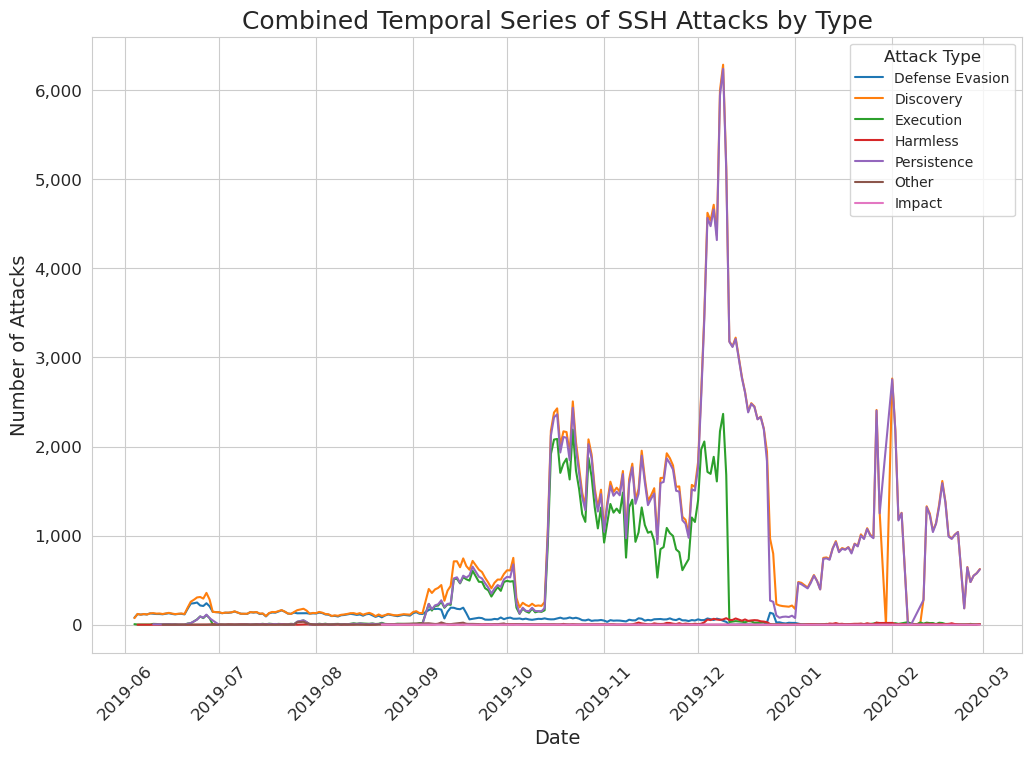
\includegraphics[width=\textwidth]{../figures/plots/section1/combined_temporal_series_of_ssh_attacks_by_type.png}
                \caption{Temporal Series of SSH Attacks}
                \label{fig:temporal-analysis}
            \end{minipage}
            \hfill
            \begin{minipage}[c]{0.47\textwidth}
                \centering
                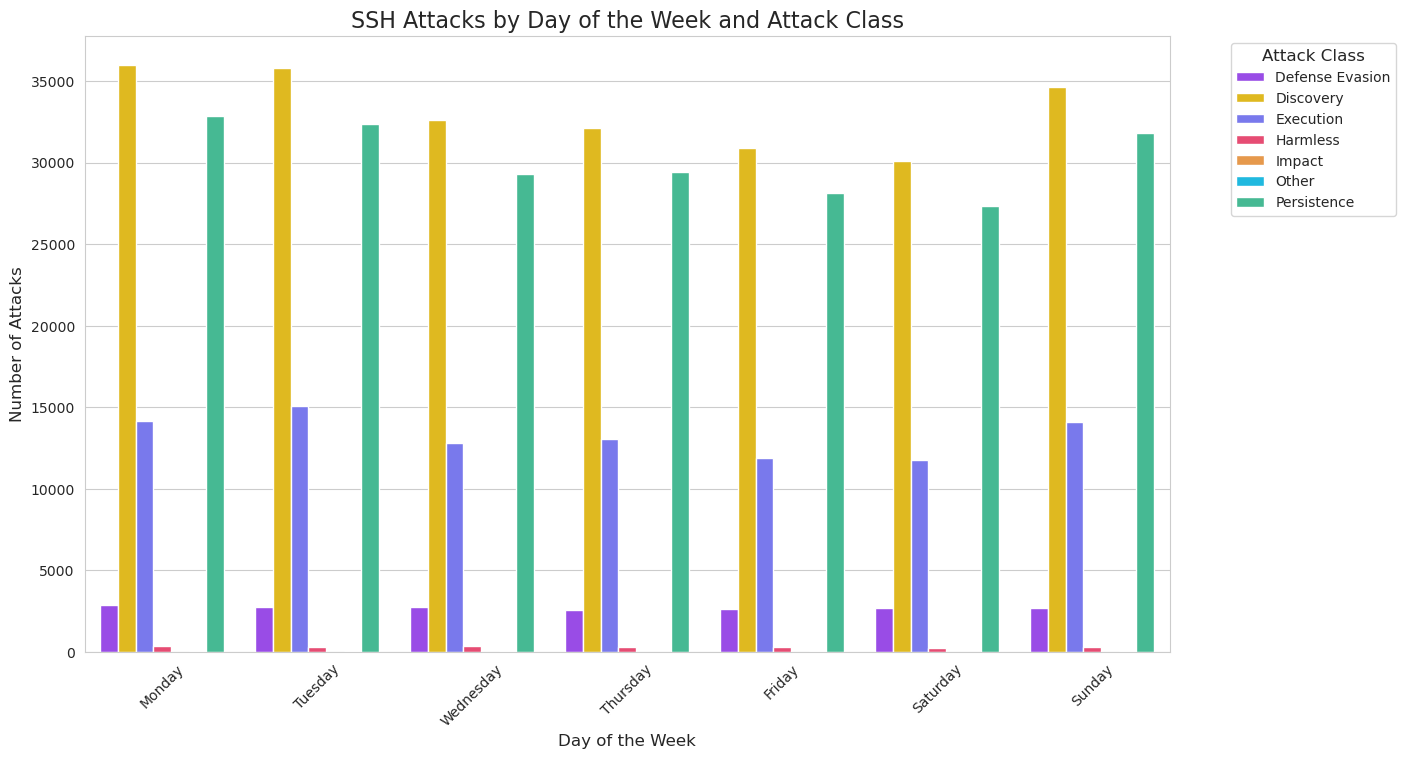
\includegraphics[width=\textwidth]{../figures/plots/section1/ssh_attacks_by_day_of_the_week_and_attack_class.png}
                \caption{Attacks by the day of the week}
                \label{fig:attacks-day-of-the-week}
            \end{minipage}
        \end{figure}

        
        Our dataset spans from June 2019 to March 2020, revealing a notable concentration of attacks between mid-October 2019 and January 2020.

        Further analysis was conducted on the distribution of sessions across various temporal dimensions (months, days of the week, etc.), but no significant patterns were identified.
        
        % TODO: say that those images can be seen in the Appendix

    \subsection{Common Words Analysis}
    
        The analysis of common words within the attack sessions provides insights into frequently utilized commands and keywords. These elements are pivotal for understanding attacker behavior and informing model training for detecting attack intents. 

        To visualize and analyze the most frequent words, two approaches were used: 
        
        \vspace{0.2em}

        \begin{itemize}
        
            \item \textbf{Word Cloud Visualization}: A word cloud (Figure~\ref{fig:word-cloud}) was generated to represent the most common words in the dataset. Commands like \texttt{grep}, \texttt{cat}, \texttt{echo}, and \texttt{rm} dominate the word cloud, highlighting their frequent usage in attack sessions.
            
            \vspace{0.2em}

            \item \textbf{Top 20 Most Common Words Bar Plot}: A bar plot (Figure~\ref{fig:common-words}) showcases the top 20 most frequent words, ordered by their frequency. This plot provides more quantitative detail, revealing the high occurrence of commands such as \texttt{grep} (over 1.2 million occurrences) and \texttt{cat} (over 1 million occurrences). Other significant commands include \texttt{echo}, \texttt{rm}, \texttt{uname}, and \texttt{name}. These commands are commonly associated with file manipulation, string searching, and process information, which are typical in malicious activities.
            
        \end{itemize}
        
        \vspace{0.2em}

        The combination of these visualizations supports the identification of commonly used commands and their potential roles in attack sessions. 
        
        \begin{figure}[h]
            \centering
            \begin{minipage}[c]{0.47\textwidth}
                \centering
                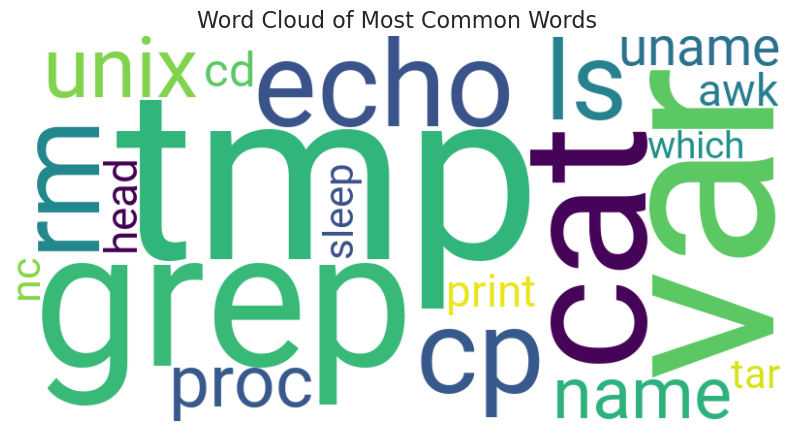
\includegraphics[width=0.95\textwidth]{../figures/plots/section1/word_cloud_of_most_common_words.png}
                \caption{Word Cloud of Most Common Words}
                \label{fig:word-cloud}
            \end{minipage}
            \hfill
            \begin{minipage}[c]{0.47\textwidth}
                \centering
                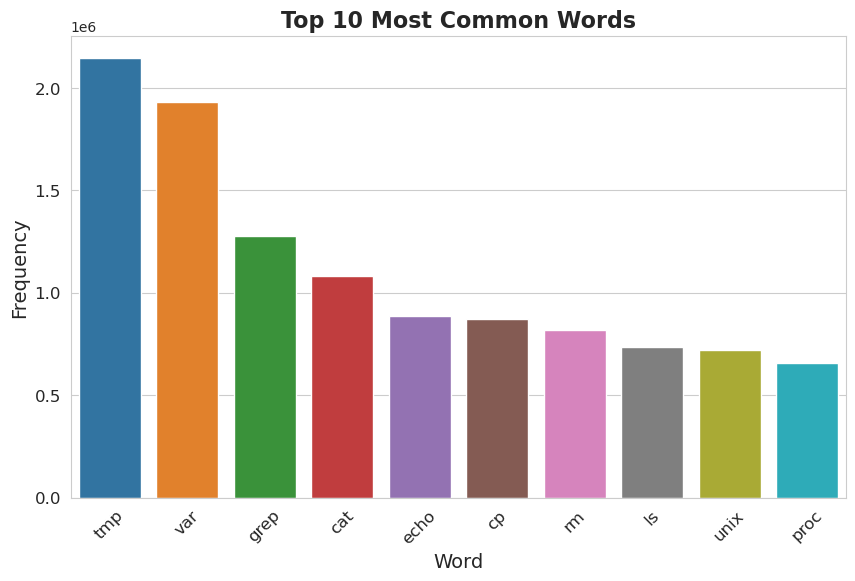
\includegraphics[width=0.95\textwidth]{../figures/plots/section1/top_10_most_common_words.png}
                \caption{Top 20 Most Common Words}
                \label{fig:common-words}
            \end{minipage}
        \end{figure}
        
    \vspace{-0.3cm}

    \subsection{Intent Analysis}
    
        This section presents an analysis of different intents identified in attack sessions and their relationships. Our analysis reveals distinct patterns in both the frequency of individual intents and their co-occurrence relationships, providing valuable insights into attacker behavior patterns.

        Figure \ref{fig:occurrences-of-each-intent} illustrates the frequency distribution of different intents in our dataset. The analysis reveals that Discovery and Persistence are the most prevalent intents, with approximately 200,000 occurrences each. This suggests that attackers primarily focus on reconnaissance activities and establishing long-term presence in the targeted systems. Execution intent appears as the third most common, with roughly 100,000 occurrences, indicating a significant number of attempts to run malicious code. Defense Evasion shows notably fewer occurrences (around 20,000), while Harmless, Other, and Impact intents are relatively rare in the dataset.

        The co-occurrence heatmap (Figure \ref{fig:co-occurrence-heatmap-of-intents}) reveals significant patterns in how different intents interact within attack sessions. Several key observations emerge:
        
        \vspace{0.2em}

        \begin{itemize}
        
            \item The strongest co-occurrence relationship exists between Discovery and Persistence (211,281 co-occurrences), suggesting that attackers often combine reconnaissance activities with attempts to maintain system access.

            \vspace{0.2em}

            \item Execution shows strong correlations with both Discovery (92,279) and Persistence (91,576), indicating that malicious code execution frequently accompanies both system discovery and persistence establishment attempts.

            \vspace{0.2em}

            \item Defense Evasion exhibits moderate co-occurrence with Discovery (18,825) and minimal correlation with other intents, suggesting that evasion techniques are primarily employed during reconnaissance phases.

            \vspace{0.2em}

            \item Harmless, Impact, and Other intents show minimal co-occurrence with other categories (with values mostly under 20 co-occurrences). This isolation pattern is partially explained by their low frequency in the dataset: Harmless with 2,206 occurrences, Impact with only 27 occurrences, and Other with 327 occurrences. These numbers represent a small fraction of the total recorded intents, naturally limiting their potential for co-occurrence with other intent types.
            
        \end{itemize}
        
        \vspace{-0.2cm}
        
        \begin{figure}[h]
            \centering
            \begin{minipage}[c]{0.47\textwidth}
                \centering
                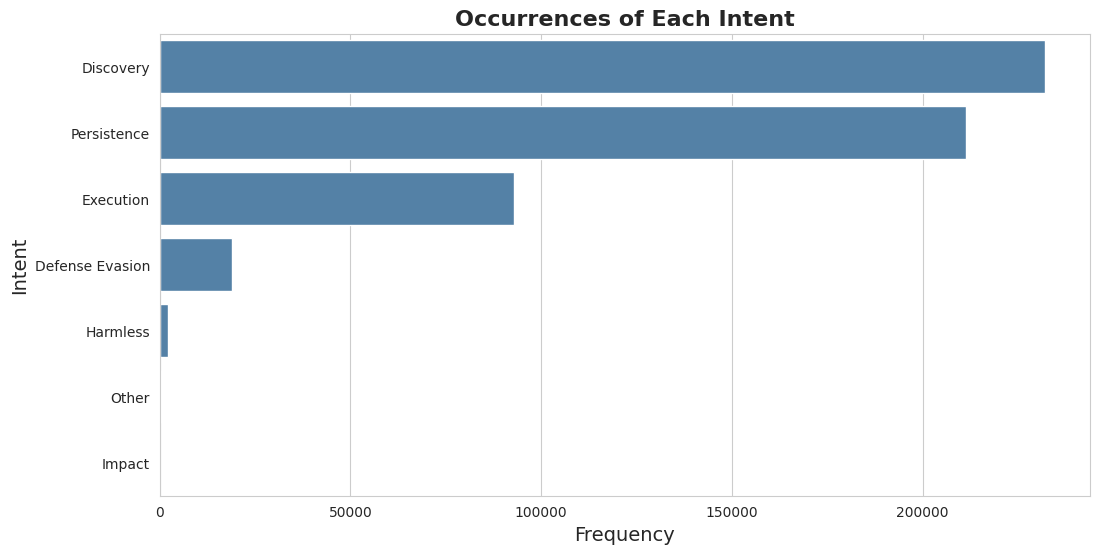
\includegraphics[width=\textwidth]{../figures/plots/section1/occurrences_of_each_intent.png}
                \caption{Occurrences of each Intent}
                \label{fig:occurrences-of-each-intent}
            \end{minipage}
            \hfill
            \begin{minipage}[c]{0.47\textwidth}
                \centering
                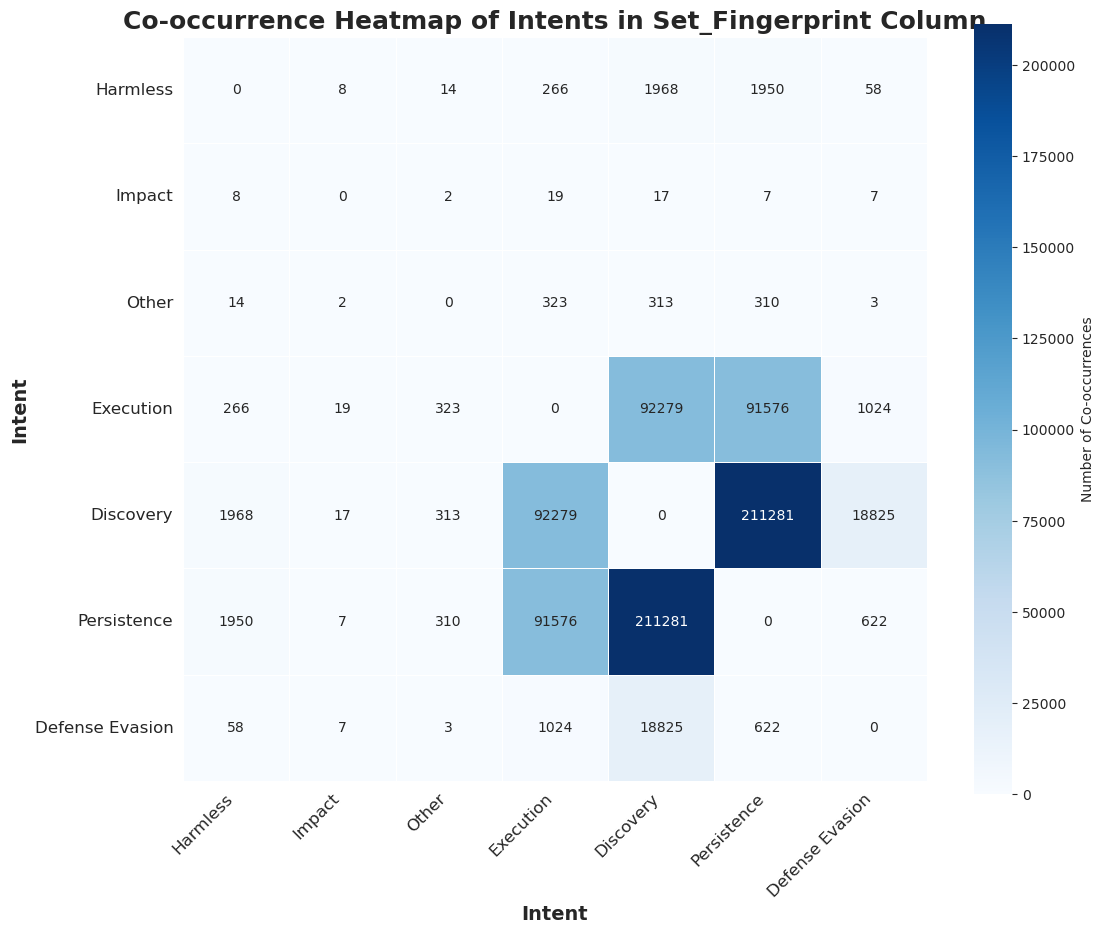
\includegraphics[width=\textwidth]{../figures/plots/section1/co-occurrence_heatmap_of_intents_in_set_fingerprint_column.png}
                \caption{Co-Occurrence Heatmap of Intents}
                \label{fig:co-occurrence-heatmap-of-intents}
            \end{minipage}
        \end{figure}

        These findings highlight common attack patterns where adversaries typically begin with discovery operations, followed by persistence establishment and execution of malicious code. This understanding can inform the development of detection strategies and defensive measures, particularly focusing on the most common intent combinations.
        
    \subsection{Session Analysis}

        The session analysis aims to understand the structural characteristics of the attack sessions in the dataset. This is accomplished through two visualizations: the Empirical Cumulative Distribution Function (ECDF) plots and the distribution of the number of words per session. The ECDF plots in Figure~\ref{fig:ecdf_sessions} provide insights into the distribution of the number of characters and words across all sessions. 
        
        \vspace{0.2em}
        
        \begin{itemize}
        
            \item The ECDF for characters indicates that the majority of sessions have fewer than $10^3$ characters, with a sharp increase between $10^2$ and $10^3$ characters. This suggests a high concentration of relatively short sessions.
            
            \vspace{0.2em}
            
            \item The ECDF for words shows a similar trend, with most sessions containing fewer than $10^2$ words. The distribution reflects the concise nature of many attack sessions, potentially focusing on executing a limited number of commands.
            
        \end{itemize}
        
        \vspace{0.2em}

        \clearpage
        
        \begin{figure}[h]
            \centering
            \begin{minipage}[c]{0.47\textwidth}
                \centering
                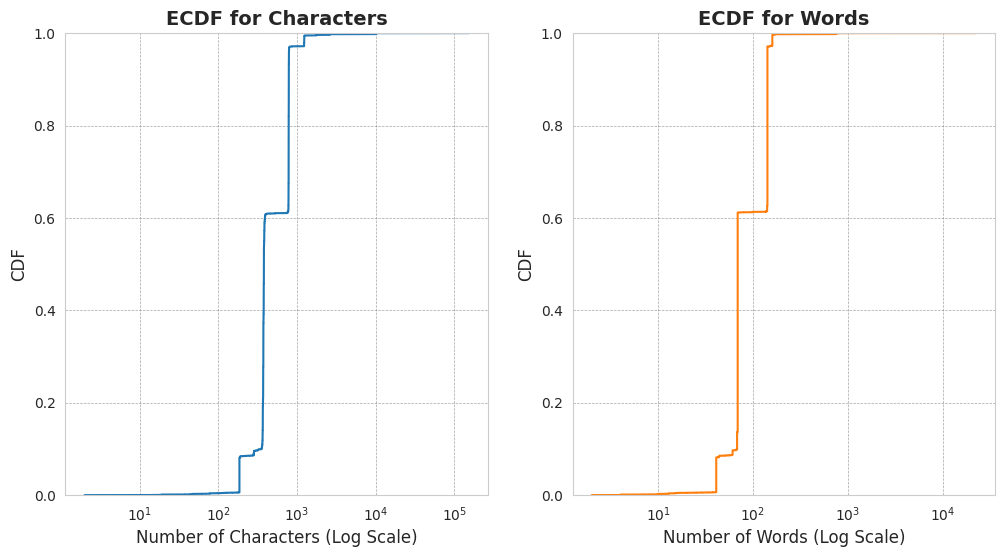
\includegraphics[width=\textwidth]{../figures/plots/section1/ecdf_for_characters_and_for_words.png}
                \caption{ECDF for Characters and Words in Sessions}
                \label{fig:ecdf_sessions}
            \end{minipage}
            \hfill
            \begin{minipage}[c]{0.47\textwidth}
                \centering
                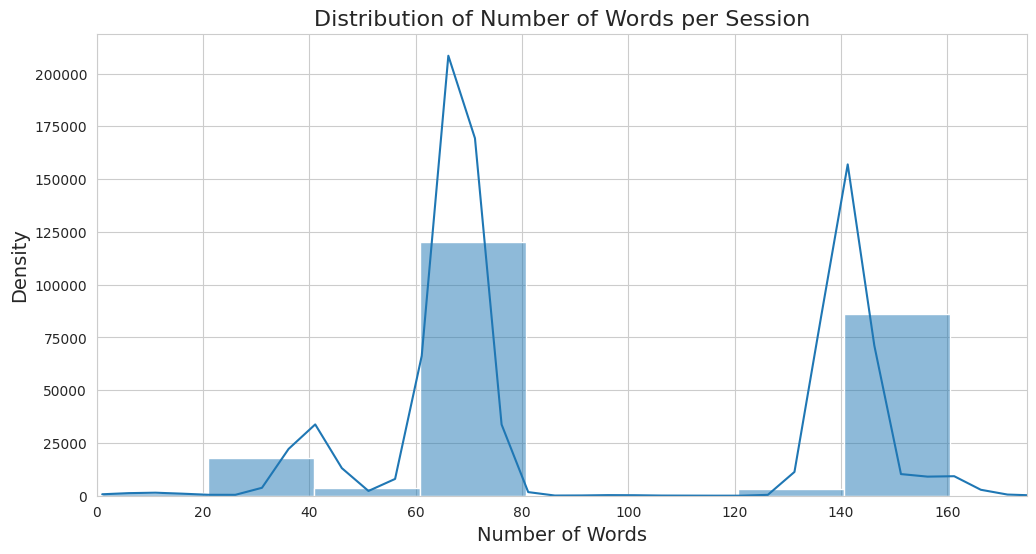
\includegraphics[width=\textwidth]{../figures/plots/section1/distribution_of_number_of_words_per_session_limited.png}
                \caption{Distribution of the Number of Words per Session}
                \label{fig:word_distribution}
            \end{minipage}
        \end{figure}
        
        \vspace{-0.35cm}

        Figure~\ref{fig:word_distribution} illustrates the density distribution of the number of words per session. Key observations include:
        
        \begin{itemize}
        
            \item The distribution is bimodal, with two distinct peaks. This likely reflects different categories of sessions, such as exploratory attacks with a larger number of commands versus simpler, targeted attacks with fewer commands.
            
            \vspace{0.2em}
            
            \item The majority of sessions have fewer than 100 words, reinforcing the compactness observed in the ECDF plots.
            
            \vspace{0.2em}
            
            \item Outliers with higher word counts likely represent complex sessions, potentially involving multiple stages or more sophisticated attack strategies.
            
        \end{itemize}

        The relevance of these plots lies in their ability to provide a foundational understanding of session structure, which is critical for feature engineering and model development. Shorter sessions may correspond to quick, automated attacks, while longer sessions might represent manual or multi-step intrusions. These insights can inform the design of models by emphasizing features tailored to the varying lengths and complexities of sessions, ultimately improving detection accuracy.

    \subsection{Text Representation}

        To enable further analysis of the dataset, the initial textual data was transformed into numerical representations. This step is essential for applying machine learning techniques, as numerical formats are required for model training and evaluation. Two widely used text representation techniques were employed:

        \begin{itemize}
        
            \item \textbf{Bag of Words (BoW)}: This technique represents each session as a vector where each dimension corresponds to a specific word, and the value represents the frequency of that word in the session. While simple and interpretable, BoW does not capture the importance or uniqueness of words across the dataset.
            
            \vspace{0.3em}
            
            \item \textbf{Term Frequency-Inverse Document Frequency (TF-IDF)}: This method extends BoW by weighting the word frequencies based on their inverse document frequency, thereby emphasizing words that are important within a session but less frequent across all sessions. This approach helps us, through the "min\_df" parameter to remove from the initial dataset, the words that have a very low frequency. In our case, we set the "min\_df" parameter to 0.01, which means that words that appear in less than 1\% of the sessions are removed. In this way the features are reduced from 300.000 to 90.
            
        \end{itemize}

        Figure~\ref{fig:bow} and Figure ~\ref{fig:tf-idf} illustrate the transformed datasets using the BoW and TF-IDF techniques, respectively.
        
        The TF-IDF representation was chosen for further analysis as it captures meaningful patterns by emphasizing word relevance, ensuring that subsequent analyses focus on the most distinctive features of each session, thereby enhancing the effectiveness of machine learning models in identifying patterns and predicting intents.

        \begin{figure}[H]
            \centering
            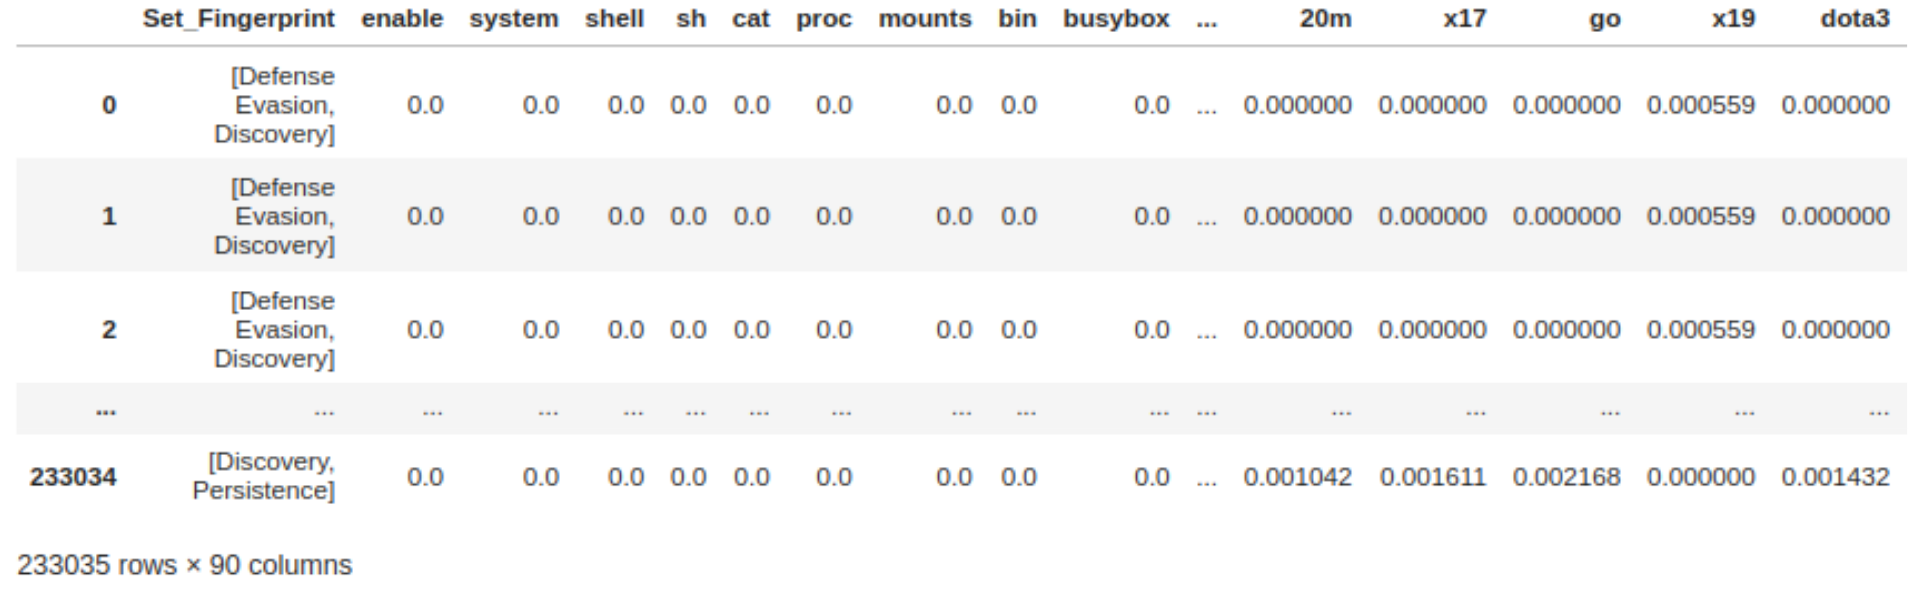
\includegraphics[width=0.80\textwidth]{../figures/others/dataset_bow_1.png}
            \vspace{-0.3cm}
            \caption{Bag-of-Words}
            \label{fig:bow}
        \end{figure}
        
        \vspace{-0.5cm}
        
        \begin{figure}[H]
            \centering
            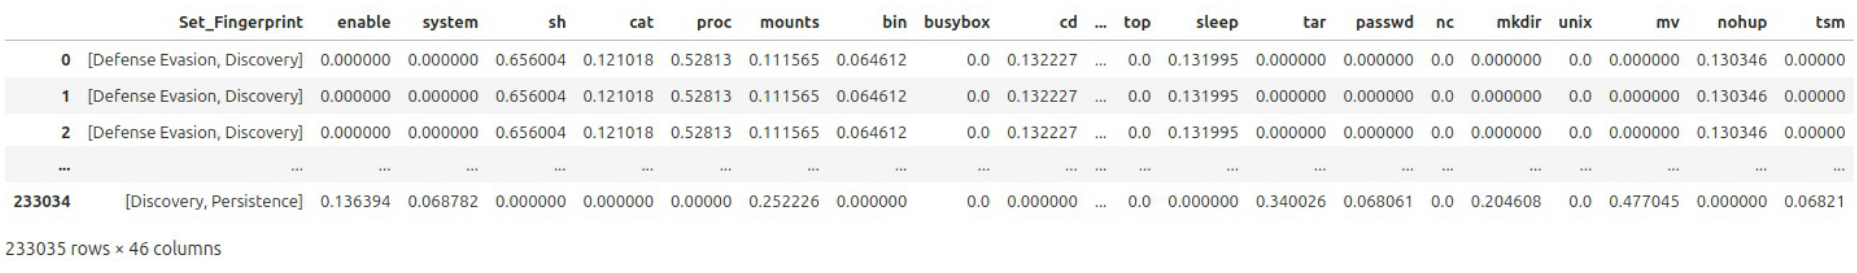
\includegraphics[width=0.80\textwidth]{../figures/others/dataset_tf-idf_1.png}
            \vspace{-0.3cm}
            \caption{TF-IDF}
            \label{fig:tf-idf}
        \end{figure}
